\documentclass{scrreprt}
\usepackage[english]{babel}
\usepackage[T1]{fontenc}
\usepackage{lmodern}
\usepackage{blindtext}
\usepackage[utf8]{inputenc}
\usepackage{siunitx} %For unit handling%
\renewcommand{\familydefault}{\sfdefault}
\newcommand{\unit}[1]{\ensuremath{\, \mathrm{#1}}}
\usepackage{amssymb, amsmath, cancel, ulem, graphicx, float, tabularx, multirow, bm}
\usepackage{amsmath}
\usepackage{caption}
\usepackage{subcaption}
\usepackage{mathtools}
\usepackage{tikz}
\usepackage{commath}
\usepackage{nameref}
\newcommand*\circled[1]{\tikz[baseline=(char.base)]{
            \node[shape=circle,draw,inner sep=1pt] (char) {#1};}}
\renewcommand{\phi}{\varphi}


\setcounter{secnumdepth}{5}
\setcounter{tocdepth}{5}

\author{Urs Gerber\\09-921-156 \and Gian-Luca Mateo\\11-113-545}
\date{23th of May 2013}

\title{Molar Heat Capacity}
\subtitle{Practical course report}

\begin{document}

\maketitle

\tableofcontents
\newpage

\chapter{Experiment: Molar Heat Capacity}
\section{Introduction}


\subsection{Goal of the experiment}
The goal of this experiment is to experimentally determine the ratio $\gamma = \frac{C_v}{C_p}$ of the molar heat capacity for constant volume to the molar heat capacity for constant pressure for different gases, namely Argon ($Ar$), Nitrogen ($N_2$) and Carbon Dioxide ($CO_2$). 
 
\subsection{Theory} 
The state of an ideal gas can be manipulated by adding or removing heat or work to/from the system. Two parameters can define the way a gas behaves under such manipulations, namely how much energy is needed to heat a gas for constant volume and how much energy is needed to heat it for constant pressure.
\begin{equation}
C_v = \left. \frac{\delta Q}{\dif{T}} \right\|_{V=const}
\qquad C_p = \left. \frac{\delta Q}{\dif{T}} \right\|_{p=const} 
\end{equation}
...
\
\subsubsection{Error analysis}
\begin{equation}
s_{\omega_0} = \sqrt{\frac{s_\omega^2 \omega^2 + s_\lambda^2 \lambda^2}{\omega^2+\lambda^2}}
\end{equation}
Since $\omega \gg \lambda$, $\lambda$ only has a limited effect on the value of $\omega_0$.\\

\begin{equation}
s_\gamma = 8 \pi \frac{m s_{T_0} V_0^2}{A^2 p_0 T_0^3}
\end{equation} 

\section{Experiment setup and execution}

\subsection{Used materials}
The materials used in this experiment are the following:
\begin{itemize}
\item A gas tank made of glass, $V = 5633 \unit{cm^3}$
\item A tube attached vertically to the glass, $L \approx 45\unit{cm}$, $R = 16 \unit{mm}$
\item A small metal ball, $m = 17 \unit{g}$
\item 3 gas bottles, containing $N_2$, $CO_2$ and $Ar$ respectively
\end{itemize}

\subsection{Assembly and Execution}

\section{Measurements}
\begin{figure}[H]
	\centering
  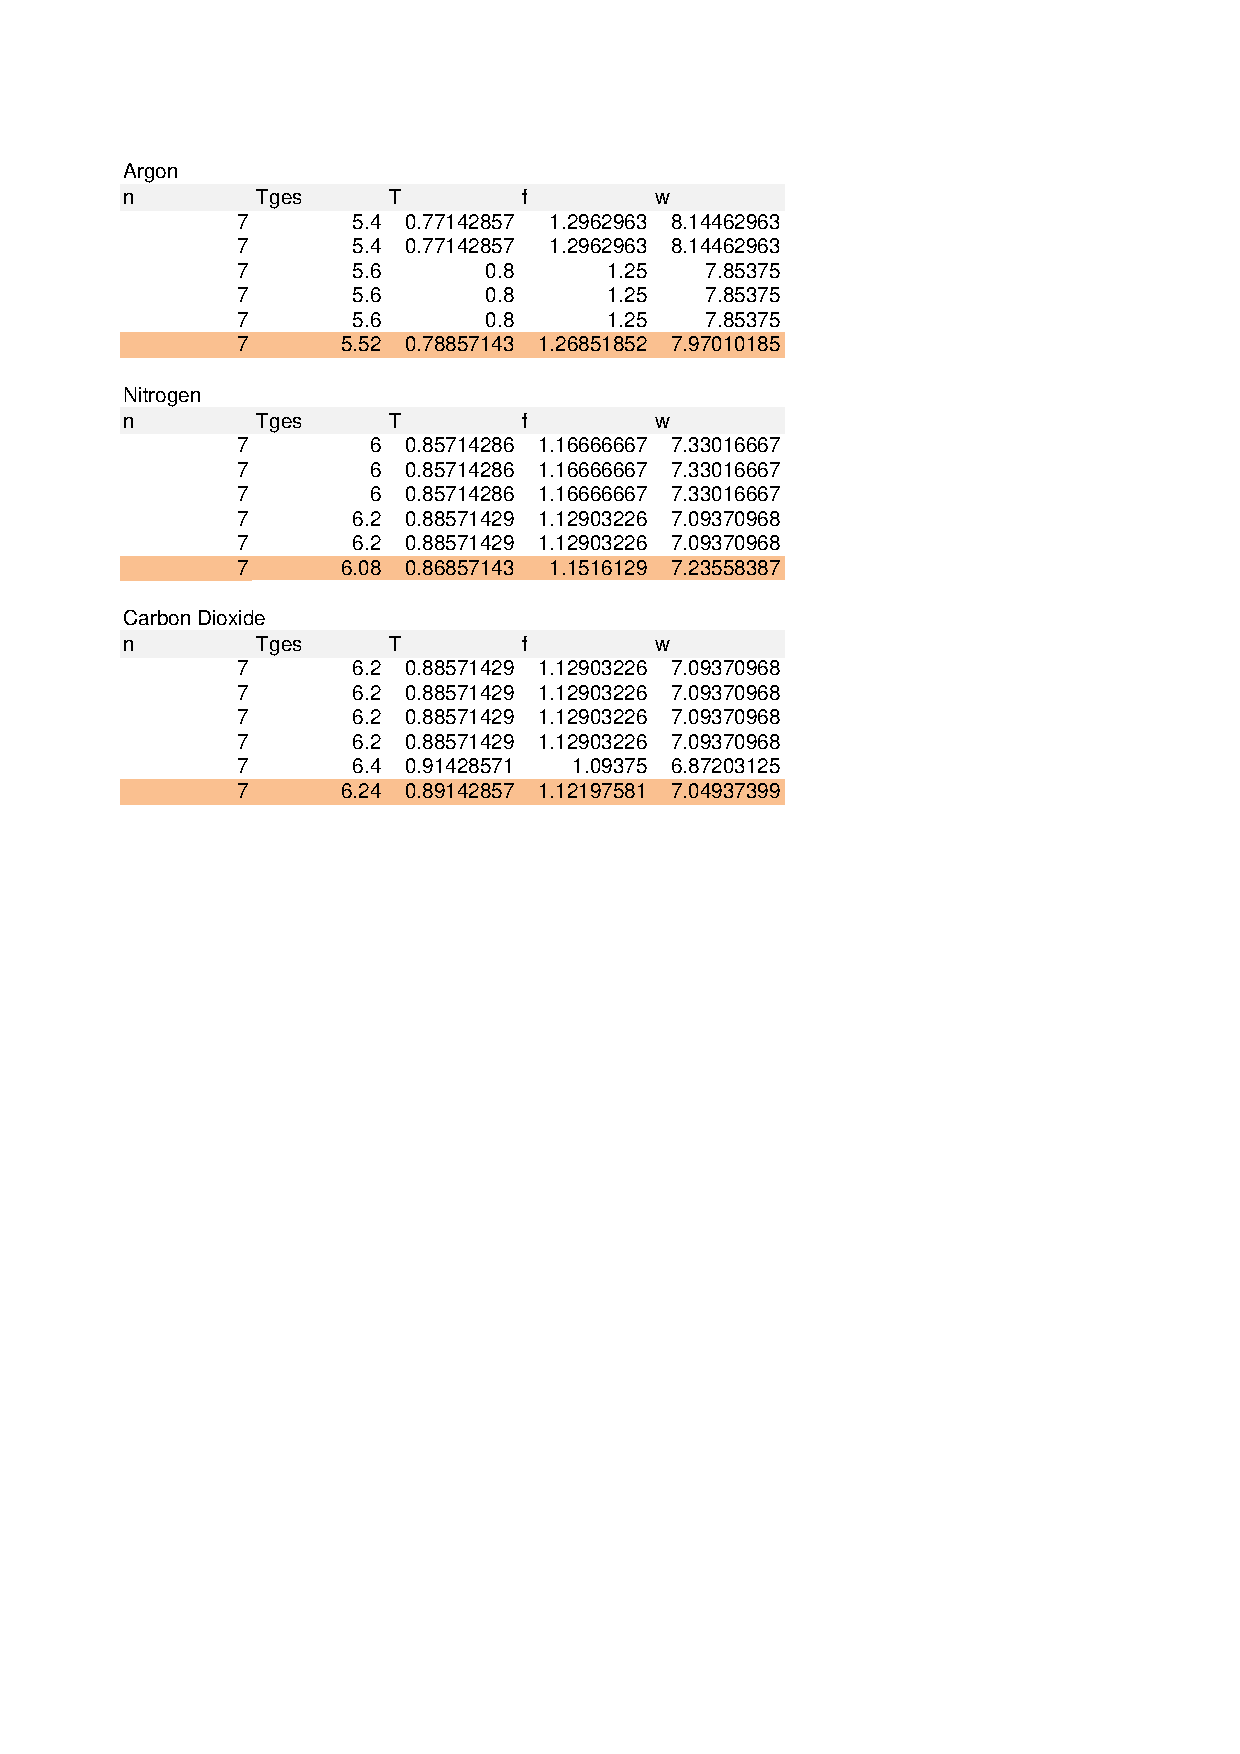
\includegraphics[width=0.7\textwidth]{diag/rawvals.pdf}
	\caption{Measured Values for the Oscillation Period of the Ball}
	\label{fig:measurement}
\end{figure}

\begin{figure}[H]
	\centering
  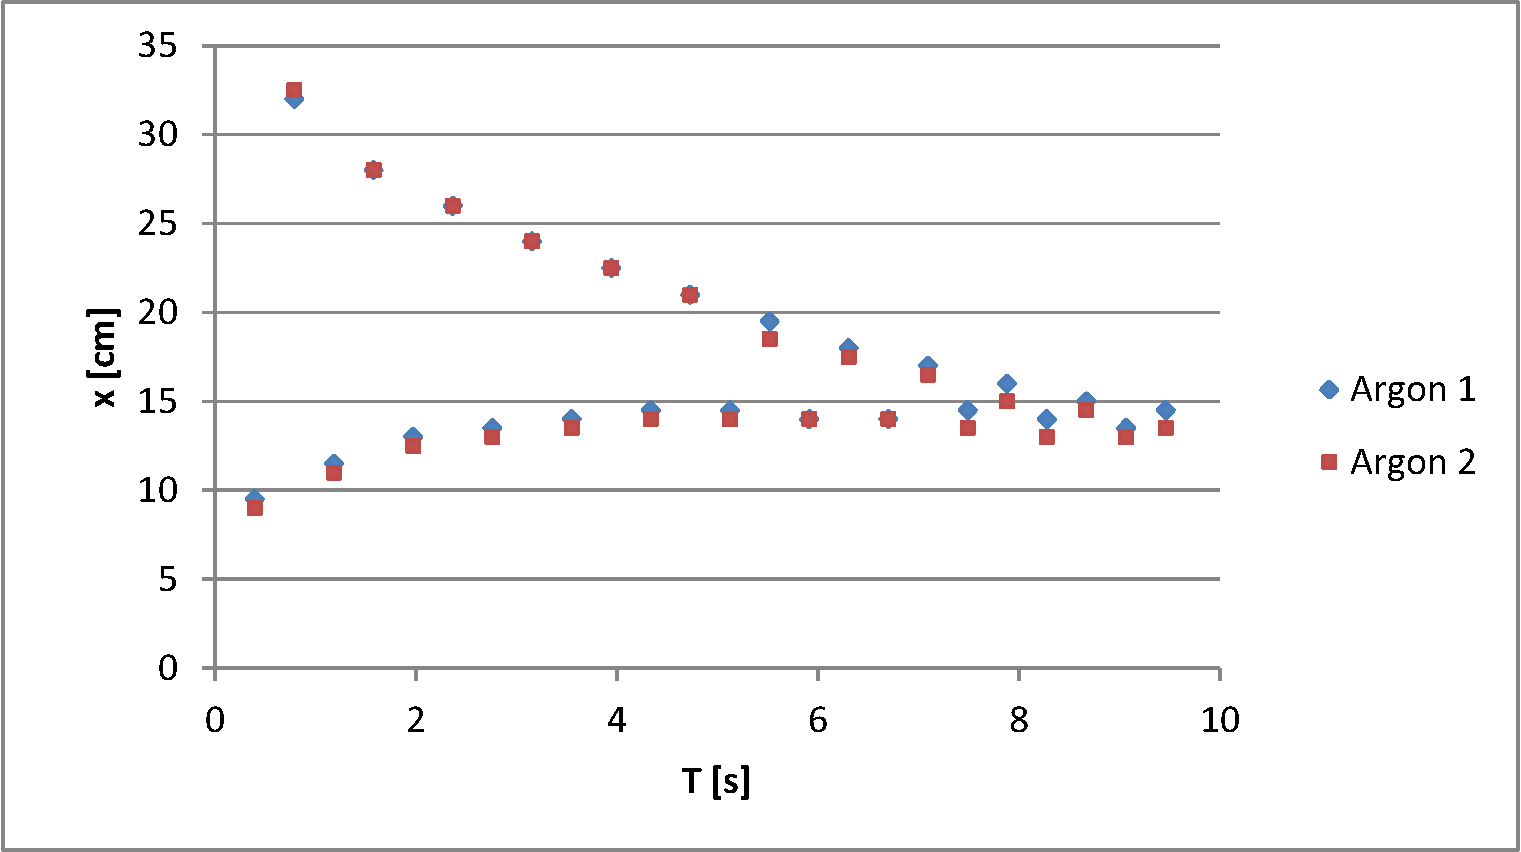
\includegraphics[width=0.7\textwidth]{diag/argon.pdf}
	\caption{Measured Oscillations of the Ball with Argon in the Tank}
	\label{fig:argon}
\end{figure}

\begin{figure}[H]
	\centering
  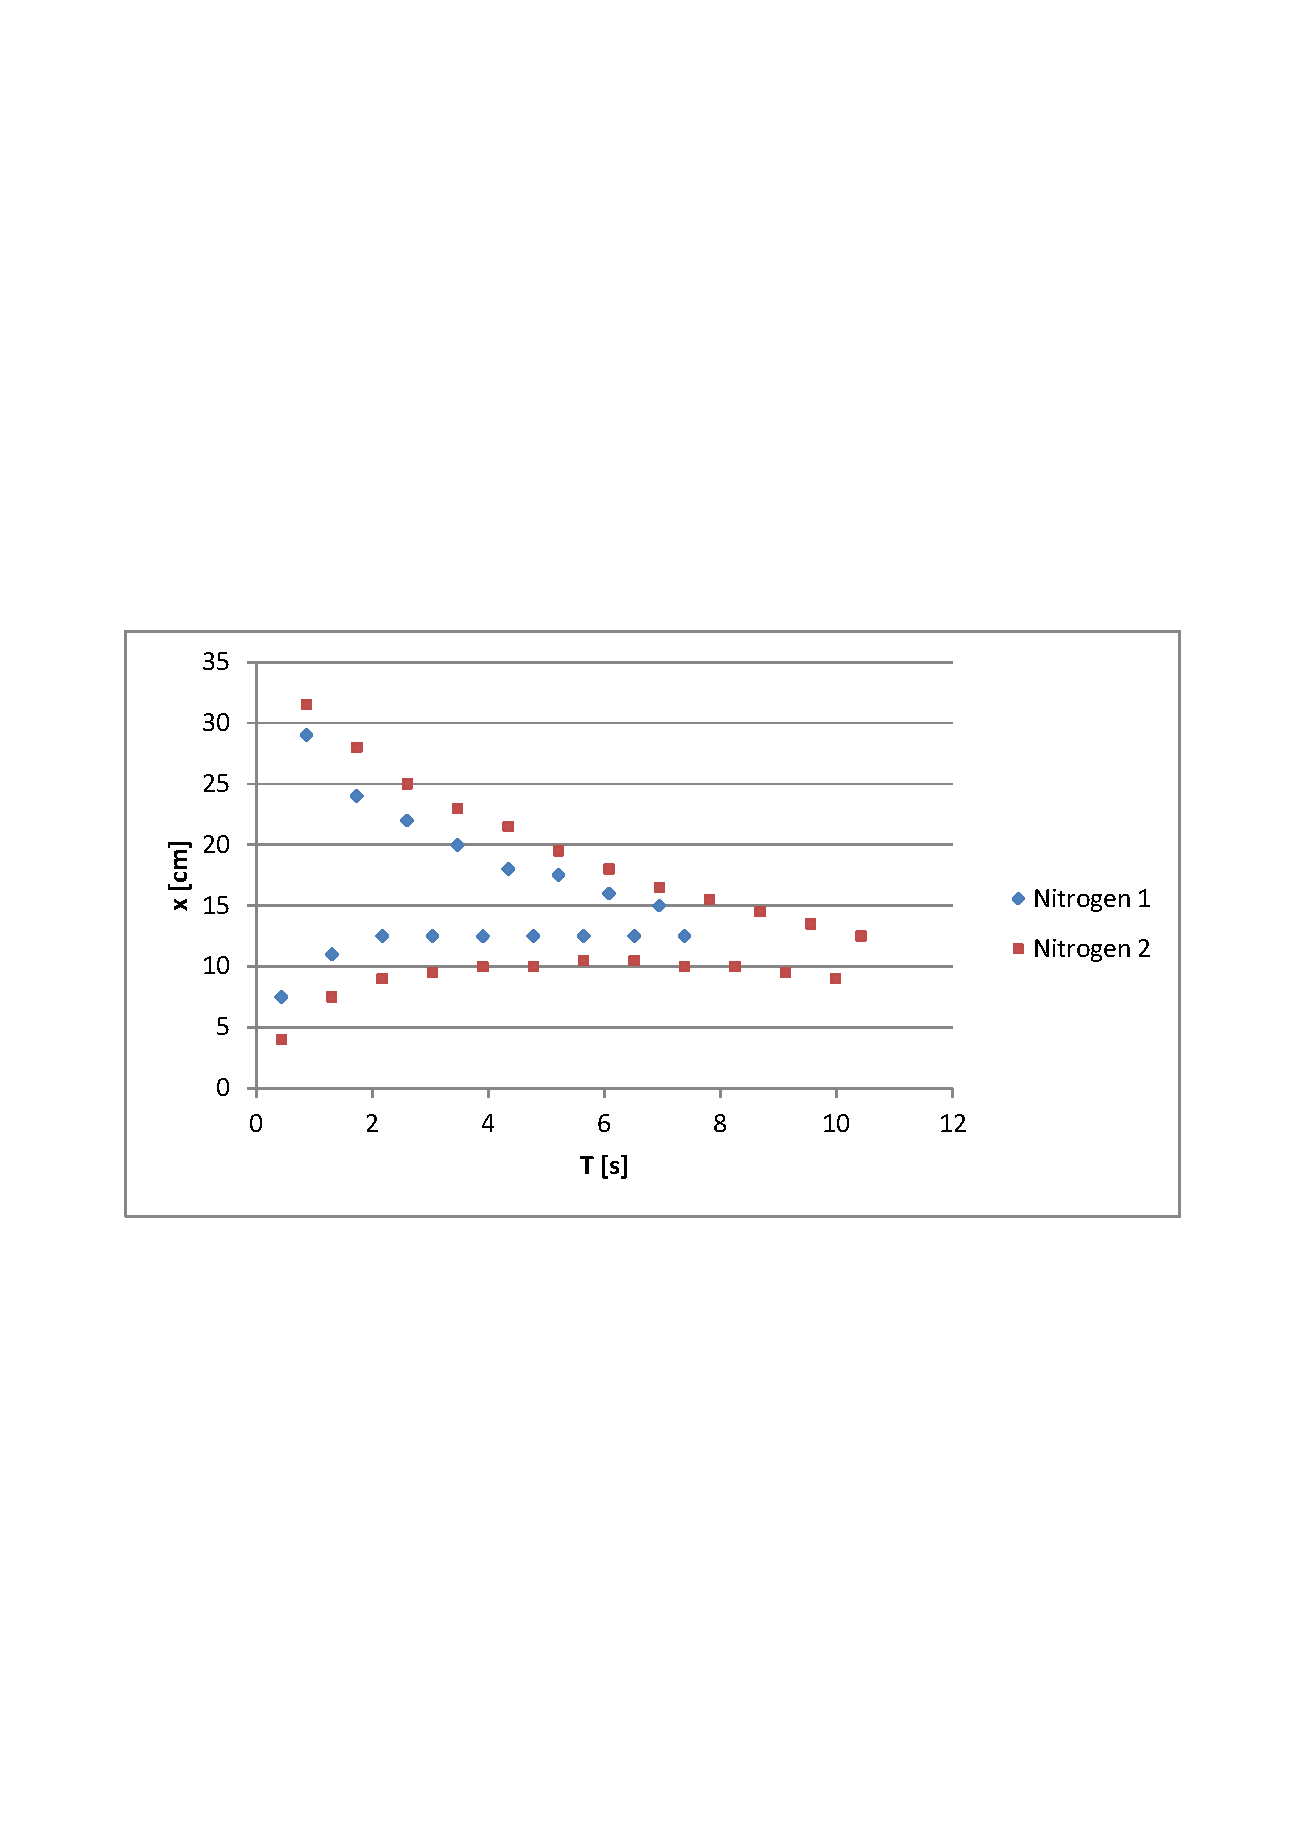
\includegraphics[width=0.7\textwidth]{diag/nitrogen.pdf}
	\caption{Measured Oscillations of the Ball with Nitrogen in the Tank}
	\label{fig:nitrogen}
\end{figure}

\begin{figure}[H]
	\centering
  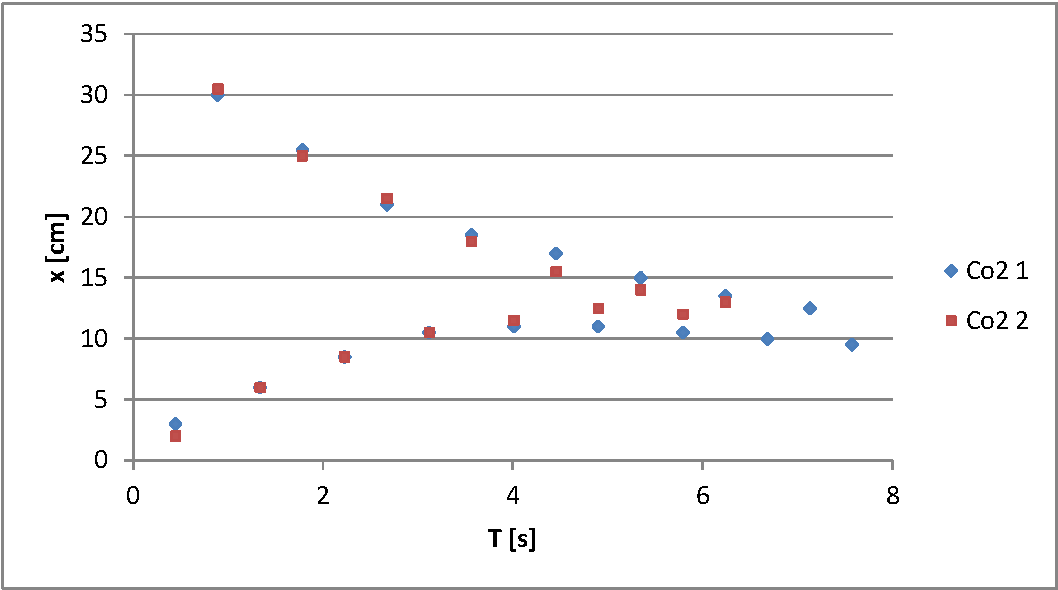
\includegraphics[width=0.7\textwidth]{diag/co2.pdf}
	\caption{Measured Oscillations of the Ball with Carbon Dioxide in the Tank}
	\label{fig:co2}
\end{figure}

\newpage
\section{Analysis and Discussion}
In order to obtain the decay coefficient $\lambda$, the graphs \ref{fig:argon} to \ref{fig:co2} need to be adjusted to fit the expected history of a damped harmonic oscillation. 

\begin{figure}[H]
	\centering
  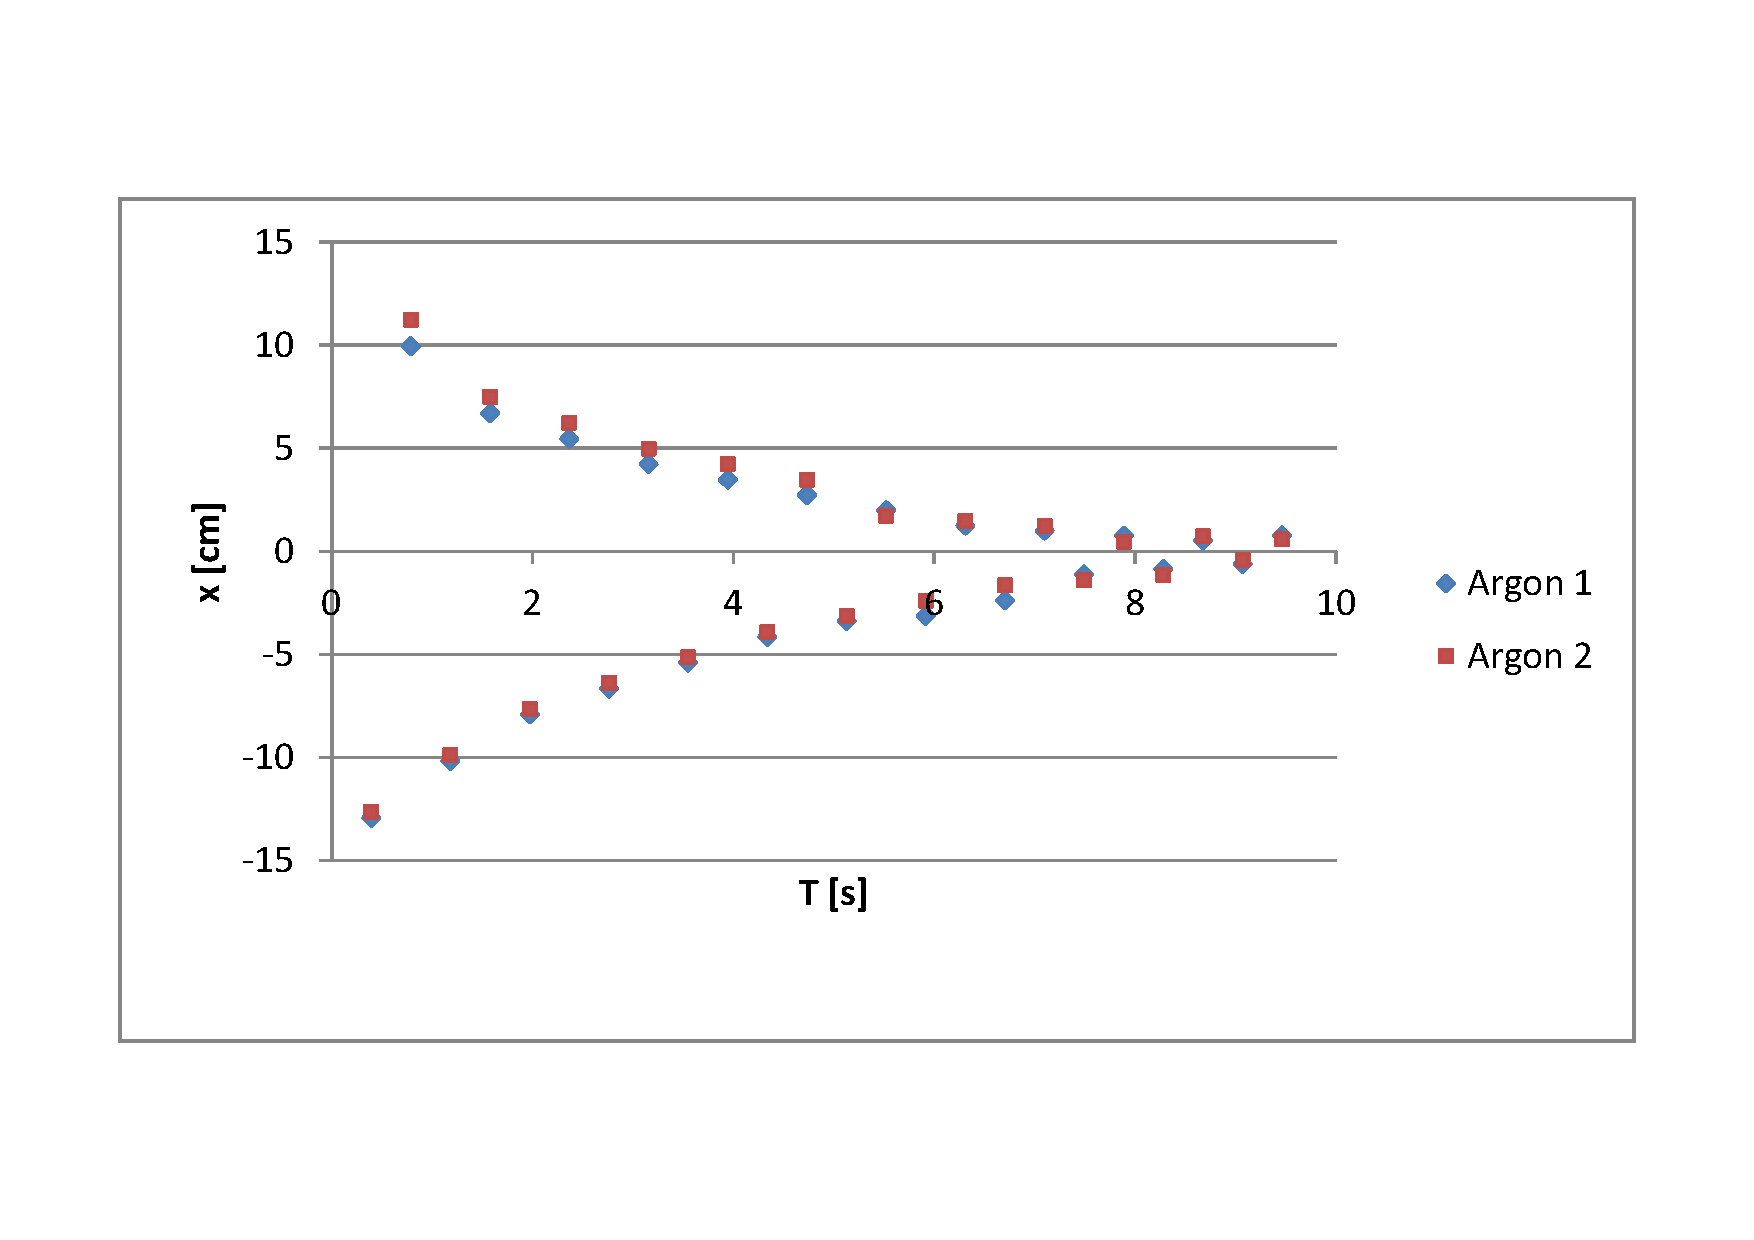
\includegraphics[width=0.7\textwidth]{diag/argon_adjusted.pdf}
	\caption{The adjusted Graph for the Tank filled with Argon}
	\label{fig:argon_adjusted}
\end{figure}

We can now exponentially fit the graph with a model of the forml $C e^{-\lambda t} + b$ and thus obtain the values for $\lambda$ and use that to calculate the frequency of the undamped oscillation $\omega_0$ using

\begin{equation}
\omega_0^2=\omega^2+\lambda^2
\end{equation}

\begin{table}[H]
\center
\begin{tabular}{|l|ccc|}
\hline
	&	$Ar$ & $N_2$		&	$CO_2$\\ \hline\hline
$T$ [$\unit{s}$] & $0.789 \pm 0.006$ & $0.869 \pm 0.006$  & $0.891 \pm 0.00571$\\\hline\hline
$\omega$ [$\unit{Hz}$] & $7.970 \pm 0.0713$ & $7.238 \pm 0.0579$ & $7.0496 \pm 0.0443$\\\hline
$\lambda$ & $0.257 \pm 0.0148$ & $0.231 \pm 0.129$ & $0.376 \pm 0.0212$\\ \hline
$\omega_0$[$\unit{Hz}$] & $7.974 \pm 0.0712$ & $7.245 \pm 0.0582$ & $7.0596 \pm 0.0443$ \\ \hline

\end{tabular}
\caption{Oscillation period $T$, oscillation amplitude decay coefficient $\lambda$, and oscillation frequencies $\omega$ (damped) and $\omega_0$ (undamped) for the different gases.}
\end{table}

To find $\gamma$ we use 

\begin{equation}
\gamma = \frac{4 \pi m V_0}{p_0 A^2 T_0^2}
\end{equation}

which yields

\begin{table}[H]
\center
\begin{tabular}{|l|ccc|}
\hline
	&	$Ar$ & $N_2$		&	$CO_2$\\ \hline\hline
$\gamma$ measured & $1.498 \pm 0.00852$ & $1.234 \pm 0.00633$  & $1.174 \pm 0.00469$\\\hline
$\gamma$ expected & $1.650$ & $1.400$ & $1.290$\\ \hline
rel. $\Delta$ & $-9.20\%$ & $-11.80\%$ & $-8.97\%$\\ \hline

\end{tabular}
\caption{Calculated $\gamma = \frac{C_p}{C_v}$ values compared to actual $\gamma$ values }
\end{table}

\subsection{Sources of error}
\label{sec:error}
Looking for possible sources of error, some were worth considering. For once, as the diameter of the ball was smaller than the inner diameter of the tube, there was always some gas flowing around the ball, which could potentially have influenced our measurements slightly. The effect of this is clearly visible in the graphs \ref{fig:argon} to \ref{fig:co2} in the form of a constant drop of the oscillation center. Furthermore, we were unable to release the ball perfectly straightly into the tube, which caused the ball to repeatedly bounce from the wall of the tube. We believe this effect caused a substantial amount of friction, thus slowing the oscillation down, which would explain our values for $\gamma$ being too low.

\section{Conclusion}


\begin{thebibliography}{9}

\bibitem{physcript13}
  Peter Wurz,
  \emph{Anleitung zum Physikpraktikum}
  FS2013

\end{thebibliography}

\end{document}
